\section{Approaches}
\label{sec:Methods}

The following section will describe the most popular methods of First Packet Authentication and how they work.

\subsection{Port-Knocking}

Port Knocking (PK) is a method used to open ports on a firewall externally and is an application that offers protection by concealment of network ports, countering port scanning, as all ports remain closed \cite{8494695}.  Usually, PK is implemented with a server-side daemon is configured to watch the firewall log for client-side connection attempts; however, it can be also be implemented at kernel level with a kernel-level packet filter \cite{kernel}, or at a higher level application level.  Note that only the packet headers are used for authentication.\\\par
It waits for a specific sequence of packets before granting access to the services behind the firewall.  The packet itself can consist of any number of packets on the transport layer or even other underlying layers and is similar to a secret handshake.  The complexity of the knock can vary immensely. 
After authentication, the firewall is temporarily reconfigured to allow communication between the client and server.  The session is kept alive after an established connection between the client and the service.
PK is stateful.  That means that no further knocking is allowed in the event of any wrong knock.  Since the zero trust approach is implemented, the remote user is not given any information as to which knock was unsuccessful, as no packets are sent to the client at any given time.\par


\subsection{Single Packet Authorization/Authentication}

Understanding Port Knocking is essential to understand Single Packet Authorization (SPA) because it is one of the most popular types of PK.
SPA was invented in the early 2000s and was commonly used for root SSH access to servers \cite{networkinsight}.\\\par

Note that the keyword 'Authorization' in this context is misleading. To explain, authorization is the process of specifying access rights to resources by specific users.  However, when establishing a connection for SSH, for example, the remote user needs to be authenticated, not authorized, and they are doing that with the first and only package sent.  Thus 'Authentication' would be more precise in this method.  However, since 'Authorization' has been widely used for this method, this paper will also resort to 'Authorization' to avoid confusion.\\\par

Similarly to PK, SPA uses a SPA server and SPA client.  However, unlike PK, where any number of knocks (and usually more than one) is used, SPA's idea is to use one encrypted knock for authentication.

The Single Packet Authorization packet has the following structure \cite{SPAwiki}:
\begin{itemize}
    \item 16 bytes of random data, renders the packet unique
    \item local username
    \item local timestamp, preventing replay attacks
    \item FireWall KNock OPerator (fwknop) version
    \item mode (access or command)
    \item desired access (or command string)
    \item MDA5 sum
\end{itemize}

Firewall Knock Operator (fwknop), developed by Michael Rash in the early 2000s \cite{SPAwiki} and is a Linux tool used to implement SPA on a system.  This, and its default configuration, is the implementation that is going to be referred to when talking about SPA.\par

\begin{figure*}[h!]
    \centering
    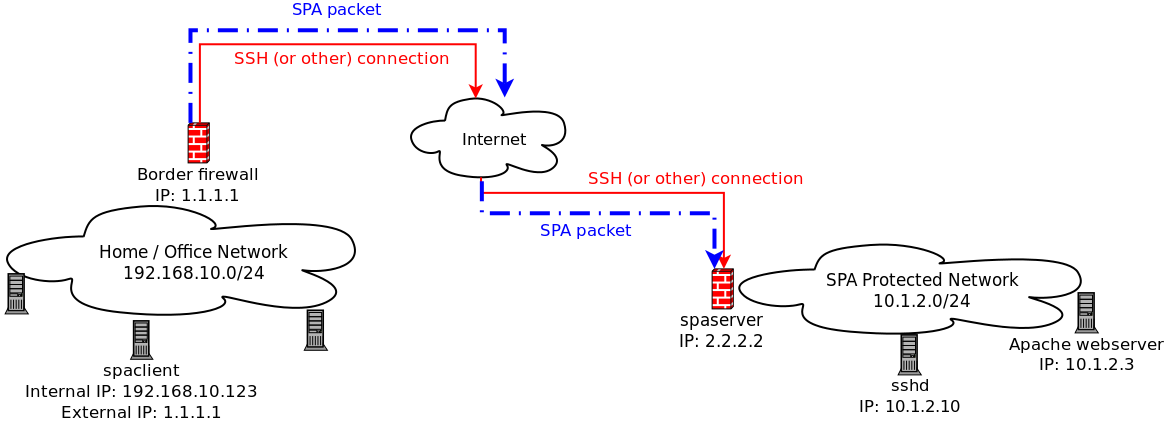
\includegraphics[width=\textwidth]{figures/fwknop_SPA.png}
    \caption{Visualization of SPA using fwknop \cite{spaimage}}
    \label{fig:fwknop_SPA}
\end{figure*}

This payload is encrypted using the MDA5 cryptographic hash function.  The cryptographic key is derived from a password (8-16 characters) entered by the user through a series of the hashing as mentioned earlier algorithm.  This results in approximately 9516 (100-bits) keys \cite{jeanquier}.  Although TCP and ICMP are also possible, SPA did not need to introduce a new protocol but uses UDP to send the authenticating knock.  SPA packets also use the packet payload to communicate authentication information, not just the packet header like PK.  The encrypted authentication data is thus then sent in a UDP packet to the specific server.  The fwknop daemon listens on UDP port 62201 or incoming packets.  When received, the daemon decrypts the data and matches it with the MDA5 checksum.  The daemon also can perform passive fingerprinting of the client and be configured only to allow access to certain machines.\\\par

Similarly to PK, after a successful knock, a connection is established, and the session is kept alive by the 'conntrack' system.  Short for 'connection tracking', conntrack is a system in the Netfilter, which makes up the basis of firewall Linux, allowing the established sessions to remain alive even though the firewall is on the default drop.  IP tables and packet filtering are part of Netfilter in Linux kernels \cite{8494695}.\par


\subsection{First Packet Authentication and Transport Access Control}

The following method to be described was developed by BlackRidge Technology and is named Transport Access Control.  Following the explicit trust principle, Transport Access Control already blocks unauthorized, anonymous traffic at the first packet.\\\par

Like SPA, Transport Access Control did not need to invent a new protocol; instead, it uses the well-established TCP/IP protocol to transmit packages.  TAC is complementary to existing security technologies. Additionally, the size of TCP/IP headers is not increased, enabling Transport Access Control to function without consuming any network bandwidth.
Each network session is authenticated at the transport layer before any access to the target and its services is provided. TAC is thus tolerant of network and port address translation and is designed to operate transparently without introducing its own port or network translation complexity. \\\par 

TAC works on the inside and outside. Externally, TAC protects against unauthorized access, port scans, and network observation.  Internally, TAC prevents viruses, malware, and rogue applications from contaminating adjacent networks \cite{blackridge}.\par

\begin{figure*}[h]
    \centering
    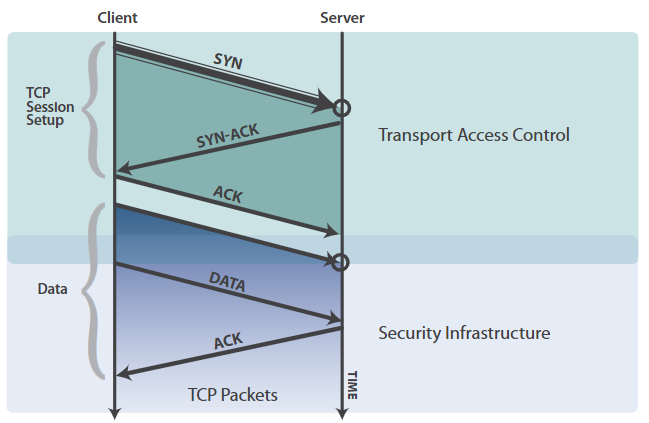
\includegraphics[width=\textwidth]{figures/TAC_arch.png}
    \caption{TCP handshake with TAC (indictated by the SYN packet arrow being framed)  \cite{blackridge}}
    \label{fig:TAC_arch}
\end{figure*}

The first step to authentication is done by generating a network identity token during the session.  This token is a 32-bit encrypted single-use object which expires after four seconds which is generated individually and cannot be reused.  Tokens are associated with identities from already existing Identity Access Management systems and credentials, like Microsoft Active Directory or the one used by Amazon Web Services. In addition, TAC uses an identity token cache to provide high scalability and low latency. \par 
They are generated for each unique entity (typically user or device) requesting access to the network.  Zero trust is established by authenticating said identity tokens and applying a security policy on the first TCP packet before any sessions with network resources can be established.  Next, an in-line virtual security gateway is established between the protected resources and the rest of the network.
Once authenticated, sessions between the server and client can be established.  If authentication fails, unauthorized traffic is rejected from the network, and again, there is no feedback to the client, preventing attackers from gathering any information about the network \cite{blackridge}. \\\par

\begin{figure*}[h]
    \centering
    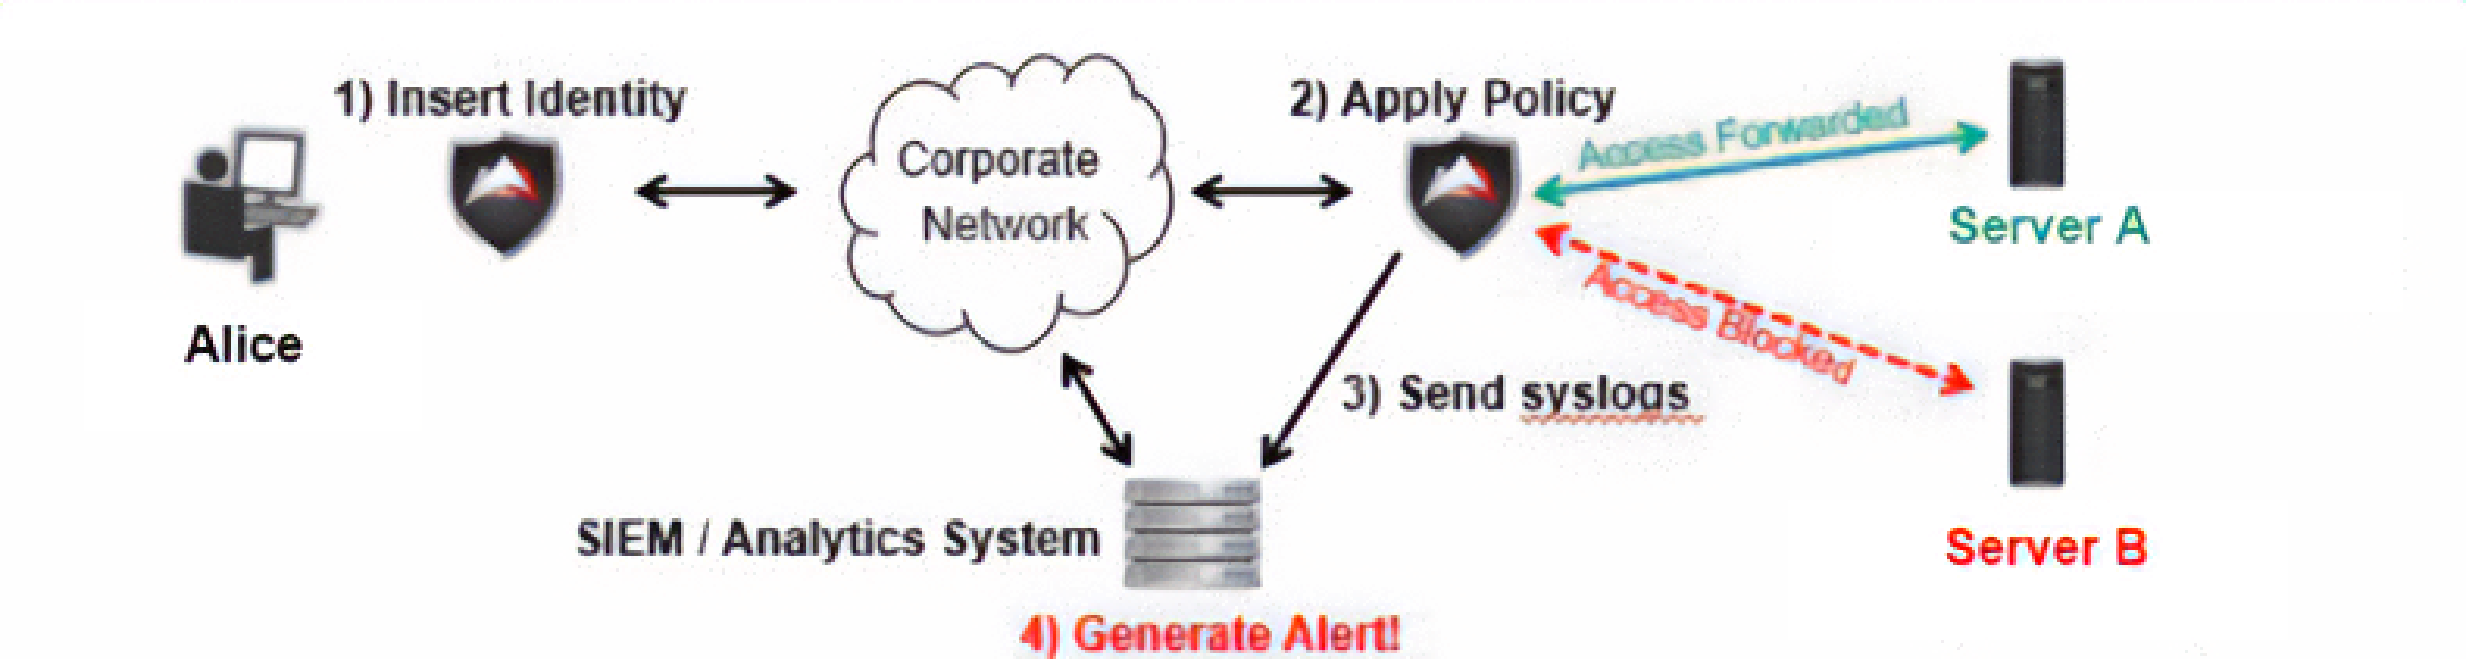
\includegraphics[width=\textwidth]{figures/alice_tac.PNG}
    \caption{TAC token authentication \cite{8494695}}
    \label{fig:alice_tac}
\end{figure*}

Figure ~\ref{fig:alice_tac} illustrates this behavior: Let there be a server A and a server B within the same network, and a user Alice who is authorized to access only server A.  A TAC gateway appliance is connected in the path between Alice and the rest of the network.  Another gateway is positioned before the protected resources.  The first gateway inserts an identity token in the first packet of the TCP connection request.  The second gateway enforces the network access policy by extracting the token, resolving it to an identity, and determining its authorizations.  If Alice attempts a connection request to server A, the gateway grants access and the connection is completed.  However, if Alice is attempting a connection request to server B, the request is denied and discarded, and Alice receives no feedback from the system in case of connection request failure.  The connection attempt is logged, and important to note is that continuous logging of all access attempts is constant with the approach of a zero trust network (i.e. not allowing any access attempts to go unmonitored).\par

When the second gateway receives a connection request, it extracts and authenticates the inserted identity token and, based on the received entity, then applies a security policy (such as forward, redirect, or discard) to the connection request.  This gateway acts as a policy enforcement point that is transparent to the rest of the system architecture. Also, it is backwards compatible with existing network technologies.\par  
If the network access token for a TCP request fails to resolve to an identity or resolves to an identity that lacks the authority to access the requested resource, the connection request is rejected without further response to the requestor.  In this way, the requestor receives no information about what sort of devices might be attacked behind the gateway, effectively cloaking the presence of a protected scientific instrument or data repository \cite{blackridge}.\\\par

In summary, TAC authenticates the first packet of a session, blocks network scans (by cloaking TAC-protected systems from unauthorized users) and filters and controls network access to resources while preserving existing concepts in cybersecurity and provides low, deterministic latency with highly scalable throughput \cite{blackridge}.\par
